% Standalone Overleaf project. Main document: main.tex. Compiler: pdfLaTeX.
% Results are discovery-only; no held-out results are included.
\documentclass[11pt,a4paper]{article}
\usepackage[margin=2.1cm]{geometry}
\usepackage[T1]{fontenc}
\usepackage[utf8]{inputenc}
\usepackage{lmodern,microtype,amsmath,amssymb,booktabs,array,longtable,graphicx}
\usepackage{enumitem,placeins,xcolor}
\usepackage[hidelinks]{hyperref}
\setlength{\parindent}{0pt}
\setlength{\parskip}{5pt}
\setlength{\emergencystretch}{3em}
\setlist{nosep,leftmargin=1.5em}
\graphicspath{{figures/}}
\newcommand{\file}[1]{\nolinkurl{#1}}
\newcommand{\head}[1]{\texttt{#1}}
\title{RI Participation in Measured Head Structures\\
\large Final Stage-4 experiment: audited discovery results}
\author{Single-hop contextual mother-of retrieval\\OLMo-2-1124-7B}
\date{27 September 2026}
\begin{document}
\maketitle

\begin{abstract}
The final experiment tests whether six additional relation-index (RI) candidates
contribute to contextual relation use and modulate five previously measured
communications. Neither the 33-head nor the 50-head retained set preserves the
full model's behaviour: the latter retains 11.5\% of the core fact-swap gap and
prefers the first chain's answer candidate in 85\% of the four-condition examples.
In this partial background, L9H16 and L1H27 improve the four-cell binding contrast
by 0.601 and 0.260 logits, respectively, but none of the 30 candidate--route
contrasts meets the predeclared effect rule. Three existing routes remain
retained, and a paired comparison of nested routes reveals a positive conditional
contribution of the RI head L18H19. Across 89 discovery families, collective RI
removal changes the fact-swap gap by 1.448 logits under mean replacement and 4.615
under paired-donor replacement, whereas the two new candidates' contributions
shrink to 0.003 and 0.006 under the latter baseline. These findings support
collective RI dependence and selective, background-dependent individual
contributions; they do not establish new serial assignments of the six candidates
to the tested routes. The 87-family held-out evaluation remains pending.
\end{abstract}

\section{Question, design and audit scope}
The question is whether RI-selected heads participate in the model's use of a
stated mother-of relation, and whether additional high-RI candidates can be
connected to known head structures. This experiment follows the frozen
\file{RI_Structure_Final_Protocol_20260926.md}, replacing the earlier greedy
reduction proposal. Its implementation is named S4.5 in the code and is also
referred to as the revised final S4.4 experiment. These are the same experiment.

\paragraph{Populations and interventions.}
The core panel uses 20 discovery families, two fact orders per family. The
extension uses all 89 discovery families, including those 20, on the original
fact-swap axis. Retained heads remain live at all test-block positions; all other
head outputs are replaced by slot/role/token-bucket means. Discovery means exclude
the tested family. MLPs, embeddings, normalization, demonstrations and any shared
answer-prefix computation remain live. A second baseline replaces excluded heads
with outputs from the paired opposite-fact prompt. The 87 held-out families have
not been evaluated in the supplied run.

\paragraph{Four-cell test.}
Let $x_{00}$ denote original facts and the original query; $x_{10}$ swaps the two
answer-side mothers; $x_{01}$ changes the query to the other affected child; and
$x_{11}$ changes both. Correct answers are $(a,b,b,a)$. The fixed-sign margin is
$M(x)=\operatorname{logit}(a)-\operatorname{logit}(b)$ at the first divergent
answer token. For a retained configuration $D$, with orders averaged within family,
\begin{align}
g_f(D)&=\mathbb{E}_o[M_D(x_{00})-M_D(x_{10})],\label{eq:gap}\\
b_f(D)&=\tfrac14\mathbb{E}_o[M_D(x_{00})-M_D(x_{10})-M_D(x_{01})+M_D(x_{11})].\label{eq:binding}
\end{align}
The reported $g$ and $b$ average these family values. Fidelity requires
$F=g(D)/g(\mathrm{full})\in[0.8,1.2]$,
$L=\mathbb{E}_f|g_f(D)-g_f(\mathrm{full})|/\mathbb{E}_f|g_f(\mathrm{full})|\leq0.2$,
and candidate accuracy within five percentage points of full in every cell and
order. Candidate accuracy compares $a$ and $b$; full-vocabulary top-token accuracy
is a separate outcome.

\paragraph{Effect rule.}
A family-level effect is coherent when its absolute mean is at least 0.1 logits
and at least 70\% of families share the mean sign. It is heterogeneous when mean
absolute effect is at least 0.1 and at least 20\% of families have absolute effect
at least 0.1. The rule is descriptive, not a significance test. Intervals use
20,000 paired family bootstrap draws with seed 20260926. All intervals in this
report are descriptive 95\% intervals.

\paragraph{What was verified.}
Run \file{s45_discovery_v2} completed under Slurm job 937878, with six RTX 2080 Ti
GPUs in three two-GPU workers; means were reused from the earlier run. The
independent CPU audit reproduced the core behaviour, candidate contrasts, route
effects, Gamma matrix, classes and intervals from 180 core behaviour rows, 360
expanded core behaviour rows and 1,600 pair-level route records. All 1,035 numeric
and consistency checks passed. The canonical freeze signature, all locally
available analysis-file hashes declared in the freeze, all declared code hashes,
and the discovery plan/pair hashes matched.

The local package does not include the original worker chunks or mean-bank
files. Its extension CSV contains 360 four-cell rows for the 20 core families,
not family-level records for the 89-family extension. Consequently, the extension
means, intervals and top-token accuracies below are taken from the signed
summary; their algebraic consistency was checked, but their full family-level
recomputation was not possible. No new model execution or held-out access was
performed for this review.

\paragraph{Gates.}
Six gate pairs from families 0, 16 and 168 passed. Saved baselines, inert hooks,
all-live equivalence, self-donor identity, question-prefix invariance,
structural-zero comparisons and disabled-control effects had zero reported
error. SDPA reconstruction error was at most $3.05\times10^{-5}$, not exactly
zero. All five full-background route means reproduced their historical anchors
within 0.05 logits; the largest drift was 0.029.

\section{Fixed structures and candidates}
The primary route definitions are:
\begin{center}\small
\begin{tabular}{@{}lp{13.8cm}@{}}
\toprule
Route & Source, intermediates and receiver \\
\midrule
T1 & L17H1 at the query-writer sites $\to$ live \{L18H18,L18H19\} $\to$ L27H6 Q at the colon.\\
T2 & L15H25 at the query child's final token $\to$ live \{L16H1,L16H21\} $\to$ L18H18 Q at the colon.\\
T3 & T1 with only L18H18 released as an intermediate.\\
T4 & L8H15 at the query fact sentence $\to$ L18H18 V, read at the colon.\\
T5 & L20H1 at the colon $\to$ L27H6 Q at the colon, an opposing route.\\
\bottomrule
\end{tabular}
\end{center}
T3 is nested in T1; these are not independent discoveries. The T2 retained-node
test additionally keeps L18H19, but its primary route anchor is the L18H18 branch.
The no-intermediate comparisons for T1--T3 are structural zeros, verified by gates.

The six additional candidates are L1H27, L11H4, L17H5, L23H10, L25H18 and L9H16.
Their selection spans different Stage-1 diagnostics: L1H27 ranks highly on target
RI, L11H4/L17H5 on query-fact first-anchor name gaps, L23H10 on the all-fact
first-anchor gap, and L25H18/L9H16 on last-anchor diagnostics. L18H19 and L8H15
are measured reference participants. The chosen background $B=C_{50}$ contains
31 of the original 59 RI-selected heads, denoted $R(B)$, and 19 non-RI heads.
It includes five of the six additional candidates; adding L9H16 creates a
51-head test configuration. C50 contains the previously identified strong-head
set, but neither all RI-selected heads nor the entire new shortlist.

\section{Retention fails because order overwhelms query selection}
Neither C33 nor C50 passes the fidelity guards (Table~\ref{tab:retention}).
The protocol therefore chooses C50 as a \emph{partial} background. C33 preserves
5.2\% of the core fact-swap gap; C50 preserves 11.5\%, with a binding contrast
of 0.752 against 5.562 in the full model. The small T masks also fail as retained
node sets. This is distinct from whether their specified communications carry
causal effect inside a broader background.

\begin{table}[htbp]\centering\small
\begin{tabular}{@{}lrrrrrl@{}}
\toprule
Mask & $g$ & $F$ & $L$ & $b$ & Candidate acc. & Guards \\
\midrule
full & +11.200 & 1.000 & 0.000 & +5.562 & 98.1\% & pass \\
empty & +0.000 & 0.000 & 1.000 & +0.000 & 50.0\% & fail \\
T1 & -0.209 & -0.019 & 1.019 & -0.028 & 50.0\% & fail \\
T2 & -0.003 & -0.000 & 1.000 & -0.000 & 50.0\% & fail \\
T3 & -0.191 & -0.017 & 1.017 & -0.018 & 49.4\% & fail \\
T4 & +0.001 & 0.000 & 1.000 & +0.000 & 50.0\% & fail \\
T5 & -0.028 & -0.003 & 1.003 & -0.003 & 50.6\% & fail \\
C33 & +0.582 & 0.052 & 0.948 & +0.442 & 50.0\% & fail \\
C50 & +1.283 & 0.115 & 0.885 & +0.752 & 50.0\% & fail \\
\bottomrule
\end{tabular}

\caption{Core retention, 20 families. Accuracy averages the eight cell--order
conditions. The guard checks every condition separately; all non-full masks fail
both gap guards and every cell--order accuracy guard.}
\label{tab:retention}
\end{table}

\begin{figure}[htbp]\centering
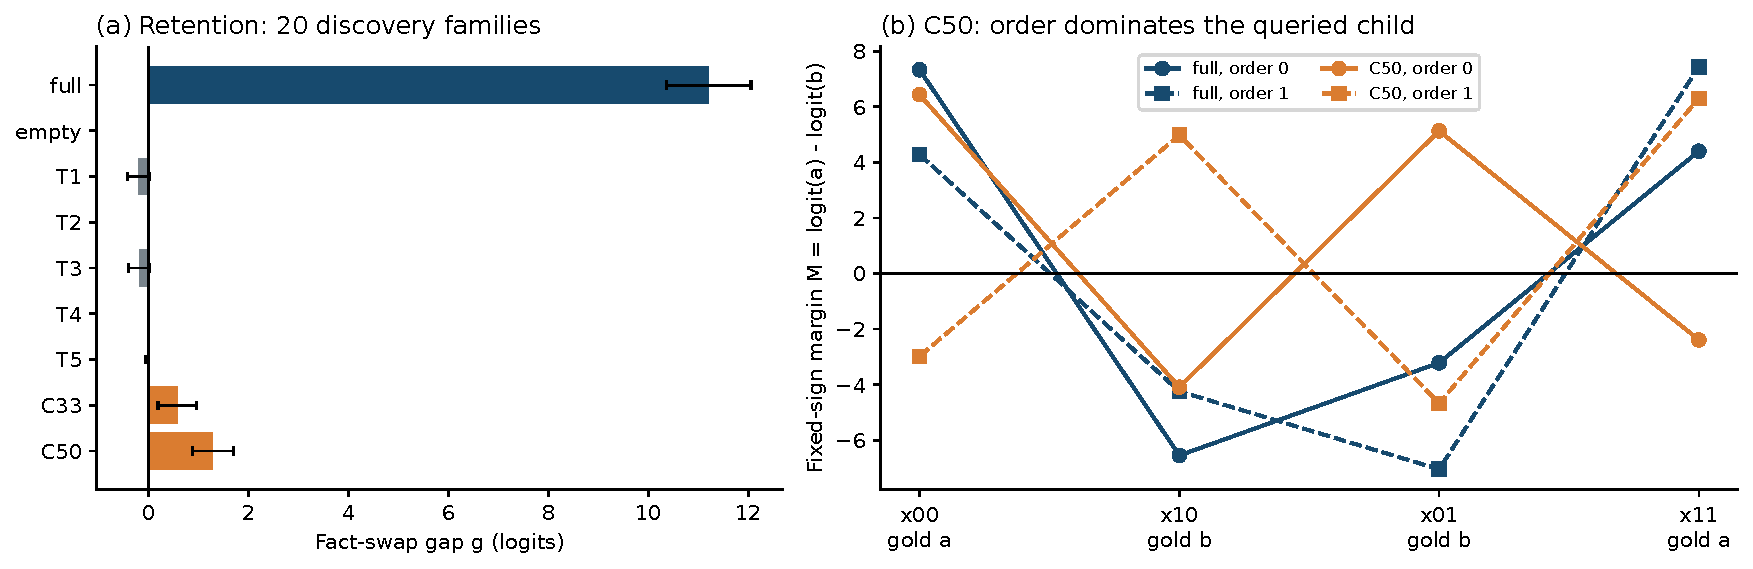
\includegraphics[width=\textwidth]{retention_and_query.pdf}
\caption{Failure of retained behaviour. (a) Fact-swap gap with family-bootstrap
intervals. (b) Four-cell margins by order: full follows the queried child, whereas
C50 largely follows the original position of the answer-side mothers. Order 0
places the originally queried chain first; order 1 places it second.}
\label{fig:retention}
\end{figure}

\paragraph{A quantified primacy pattern.}
Across the 160 core cell--order examples, C50 favours the first chain's candidate
in 85\% of cases, compared with 51.9\% for full. Yet C50's candidate accuracy is
50\%, versus 98.1\% for full. These are preferences between the two scored names,
not a claim that the vocabulary-wide prediction is always the first mother.
Changing the query moves the original-facts margin by only 1.497 logits on average,
against 10.936 in full. The behaviour retains sensitivity to names and fact order
while losing most question-conditioned discrimination.

\begin{table}[htbp]\centering\small
\begin{tabular}{@{}llrrrr@{}}
\toprule
Mask & Order & $M_{00}$ & $M_{10}$ & $M_{01}$ & $M_{11}$ \\
\midrule
full & 0 & +7.332 & -6.544 & -3.213 & +4.403 \\
full & 1 & +4.285 & -4.239 & -7.042 & +7.439 \\
C50 & 0 & +6.436 & -4.089 & +5.133 & -2.388 \\
C50 & 1 & -2.978 & +4.981 & -4.669 & +6.301 \\
\bottomrule
\end{tabular}

\caption{Mean core margins. Correct signs in column order are $(+,-,-,+)$.
The C50 sign pattern largely changes with order rather than with the question.}
\label{tab:cells}
\end{table}

The empty mask has exactly zero $g$ and $b$ on the core panel, but its margins are
not a universal constant: across families they range from $-5.496$ to $+7.547$.
Its core margins are invariant across the tested fact/query cells within each
family. On the 89-family extension, its reported gap is 0.018. Thus the empty
control shows loss of the intended contrast, not an absence of all model output
or a proof that mean replacement is a uniquely valid causal baseline.

\section{Two additional RI heads have functional effects}
For candidate $h$, compare $B_h^+=B\cup\{h\}$ with
$B_h^-=B\setminus\{h\}$ and define
$\Delta b_h=\mathbb{E}_f[b_f(B_h^+)-b_f(B_h^-)]$.
L9H16 and L1H27 pass the coherent rule (Table~\ref{tab:candidates}); both effects
are positive in every core family and in each order on average. Their
gold-oriented changes are positive on average in all four cells. The other four
candidates fall below the effect rule, rather than being exactly inactive.

\begin{table}[htbp]\centering\scriptsize
\setlength{\tabcolsep}{4pt}
\begin{tabular}{@{}lrlrrrl@{}}
\toprule
Head/group & $\Delta b$ & 95\% interval & Sign & Order 0 & Order 1 & Class \\
\midrule
L9H16 & +0.601 & [+0.518, +0.688] & 20/20 & +0.636 & +0.567 & coherent \\
L1H27 & +0.260 & [+0.215, +0.306] & 20/20 & +0.262 & +0.258 & coherent \\
L11H4 & +0.004 & [+0.002, +0.006] & 17/20 & +0.006 & +0.002 & below rule \\
L23H10 & +0.004 & [+0.001, +0.007] & 13/20 & +0.004 & +0.003 & below rule \\
L25H18 & +0.000 & [-0.004, +0.004] & 13/20 & +0.002 & -0.001 & below rule \\
L17H5 & -0.009 & [-0.015, -0.003] & 15/20 & -0.015 & -0.003 & below rule \\
RI31 jointly & +0.759 & [+0.643, +0.882] & 20/20 & +0.708 & +0.809 & coherent \\
L18H19 (ref.) & +0.247 & [+0.197, +0.303] & 20/20 & +0.240 & +0.253 & coherent \\
L8H15 (ref.) & +0.133 & [+0.103, +0.164] & 20/20 & +0.135 & +0.132 & coherent \\
\bottomrule
\end{tabular}

\caption{Core functional contributions. Sign is the number of families agreeing
with the mean sign. Reference heads and joint RI removal calibrate the candidate
measurements; they are not part of the six-candidate route search.}
\label{tab:candidates}
\end{table}

L9H16 contributes 0.601 logits, about 10.8\% of the full-model binding contrast
and 80.0\% of B's contrast. It has the largest $\Delta b$ among the individually
tested candidates and references, not necessarily among all heads in B.
Its effect exceeds either reference head's effect in this background. This is a
useful functional result even though it does not cross a candidate-accuracy
decision boundary. None of the six candidates changes candidate accuracy on the
core panel. L1H27 does, however, increase full-vocabulary top-token accuracy by
five percentage points in two conditions ($x_{10}$, order 1; $x_{11}$, order 0).

Joint removal of the 31 RI members reduces $b$ by 0.759, from 0.752 to $-0.007$.
This establishes collective dependence in the retained background. It does not
allocate that dependence to every member or only to members that were individually
strong in earlier experiments.

\section{Existing routes survive; new route assignments are not established}
\subsection{Three route effects remain retained}
T1, T3 and T4 retain coherent effects in B, at 37.2\%, 45.7\% and 53.4\% of
their corresponding full-background means (Table~\ref{tab:routes}). T2 and T5
fall below the effect rule in B. All five are weaker than in the full background.
The contrast changes the joint background throughout route capture and readout,
so it does not localize the attenuation to a particular missing selector or
downstream amplifier.

\begin{table}[htbp]\centering\scriptsize
\setlength{\tabcolsep}{3.5pt}
\begin{tabular}{@{}lrrlrrrl@{}}
\toprule
Route & Full & $B$ & 95\% interval in $B$ & Ratio & Order 0 & Order 1 & Class \\
\midrule
T1 & +1.664 & +0.618 & [+0.466, +0.766] & 37.2\% & +1.056 & +0.180 & coherent \\
T2 & +0.179 & +0.042 & [+0.026, +0.058] & 23.7\% & +0.054 & +0.031 & below rule \\
T3 & +0.859 & +0.393 & [+0.295, +0.487] & 45.7\% & +0.656 & +0.129 & coherent \\
T4 & +0.477 & +0.255 & [+0.208, +0.300] & 53.4\% & +0.380 & +0.131 & coherent \\
T5 & -0.210 & -0.019 & [-0.029, -0.008] & 8.9\% & -0.031 & -0.006 & below rule \\
\bottomrule
\end{tabular}

\caption{Route noising effects on the same 40 pairs. Ratio compares the signed
mean in B to the signed full-background mean. Effects are stronger in order 0 for
the retained routes, but remain positive in order 1.}
\label{tab:routes}
\end{table}

\paragraph{Additional finding: conditional participation of L18H19.}
T1 and T3 share source, receiver, channel and background; T1 additionally releases
L18H19 alongside L18H18. Their paired difference is
\[
 I_{T1}(B)-I_{T3}(B)=0.225\quad[0.168,0.283],
\]
positive in all 20 families. The full-background difference is
$0.805$ [$0.573,1.055$], also positive in all 20. This post hoc descriptive
comparison supports a conditional contribution of the RI head L18H19 to the
measured L17H1-to-L27H6 communication, beyond releasing L18H18 alone. It is not
an additive decomposition or a test of L18H19's necessity in the intact model.
Together with T4's L8H15 route and the reference-head functional effects, it
preserves positive evidence for known RI participants despite the unsuccessful
search for additional route assignments.

\subsection{No candidate--route pair reaches the frozen rule}
For each candidate and route,
\[
\Gamma_{h,t}=I_t(B_h^+)-I_t(B_h^-).
\]
All 30 pairs were measured; 18 have a retained route in at least one candidate
state. None passes the coherent or heterogeneous Gamma rule. The largest mean
and mean absolute Gamma both occur for L9H16--T1: $+0.0303$
[$0.0159,0.0464$] and $0.0341$, respectively, with positive signs in 17 of 20
families. Thus a small directional interaction is present descriptively, but
does not meet the planned 0.1-logit effect threshold. It should not be reported
as an exact zero or as an established new route association.

\begin{figure}[htbp]\centering
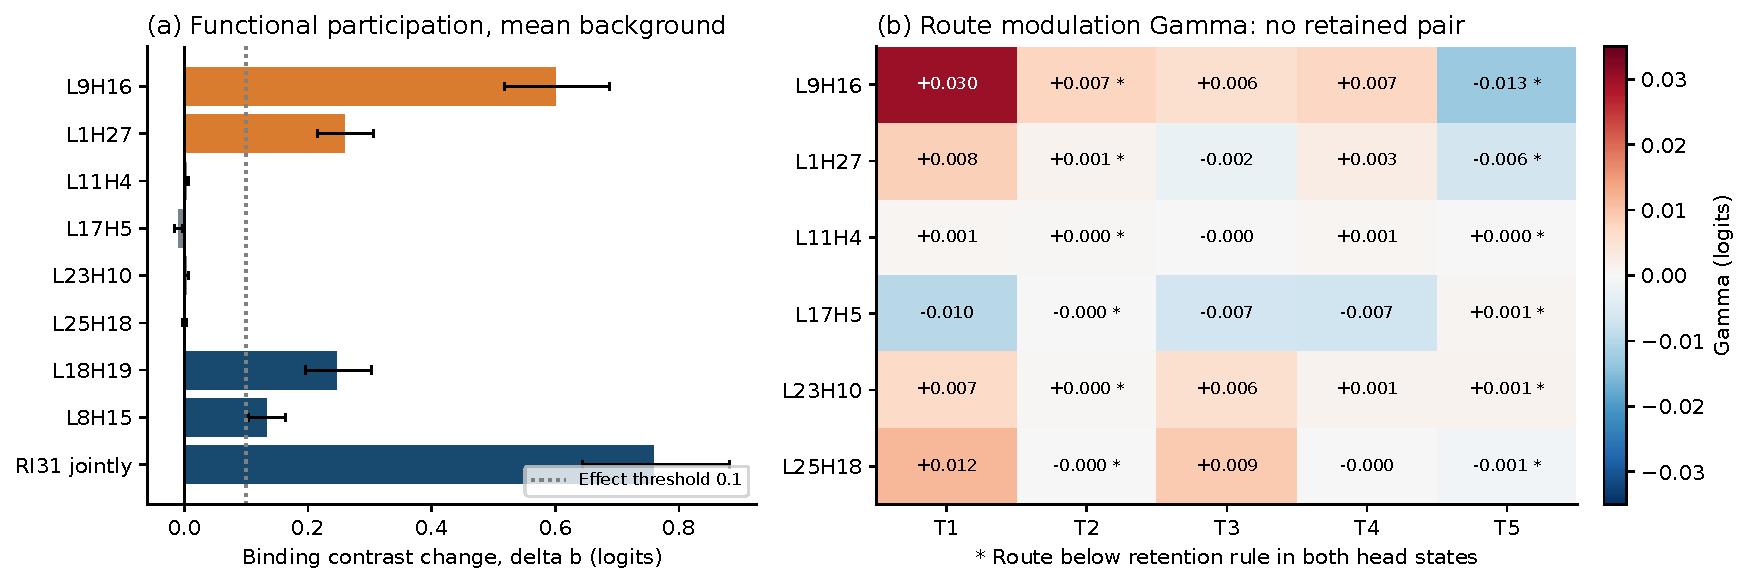
\includegraphics[width=\textwidth]{functional_and_routes.pdf}
\caption{Behavioural contribution and route modulation are distinct. (a)
Candidate/reference $\Delta b$ with family intervals; the dotted line marks the
magnitude component of the retention rule. (b) All candidate--route mean Gamma
values. Stars mark weak underlying routes in both candidate states. No pair
passes the full retention rule.}
\label{fig:function}
\end{figure}

For eligible pairs, the largest absolute Gamma is below 4.7\% of the larger
absolute route mean across the two states. This bound does not hold for weak
routes: the L9H16--T5 ratio is 41.2\% by that denominator, although its absolute
effect remains small. Two \emph{functional-only} records, L9H16 and L1H27, were
therefore selected. Stage D contained no route-pair jobs: restoration Gamma,
attachments and their matched controls were not measured. A small Gamma does
not prove that a candidate is outside a route, acts additively or in parallel,
or has no structural role. Those mechanisms remain unresolved by this run.

\section{Extension and replacement-baseline sensitivity}
The original-axis extension confirms the same pattern within the larger
discovery population (Table~\ref{tab:extension}). With means, B retains 12.0\%
of the full gap, increasing to 22.8\% when L9H16 is added. The two orders have
opposite signs. With paired donors, B has positive gaps in both orders, but
retains only 20.3\% overall. These orders are not numerically symmetric:
the gaps are 3.141 and 1.403. There is no sign reversal, which is the relevant
contrast with mean replacement.

\begin{table}[htbp]\centering\small
\begin{tabular}{@{}llrlrrr@{}}
\toprule
Configuration & Baseline & $g$ & 95\% interval & $F$ & Order 0 & Order 1 \\
\midrule
full & mean & +11.170 & [+10.623, +11.716] & 1.000 & +14.575 & +7.765 \\
empty & mean & +0.018 & [+0.000, +0.048] & 0.002 & -0.036 & +0.072 \\
B & mean & +1.342 & [+1.126, +1.567] & 0.120 & +9.937 & -7.253 \\
B & donor & +2.272 & [+1.716, +2.890] & 0.203 & +3.141 & +1.403 \\
$B-R(B)$ & mean & -0.106 & [-0.267, +0.054] & -0.009 & +5.556 & -5.767 \\
$B-R(B)$ & donor & -2.343 & [-3.043, -1.559] & -0.210 & -3.507 & -1.180 \\
B+L9H16 & mean & +2.552 & [+2.271, +2.861] & 0.228 & +10.921 & -5.816 \\
B+L9H16 & donor & +2.275 & [+1.717, +2.894] & 0.204 & +3.157 & +1.393 \\
B-L1H27 & mean & +0.790 & [+0.588, +0.997] & 0.071 & +8.954 & -7.374 \\
B-L1H27 & donor & +2.266 & [+1.708, +2.892] & 0.203 & +3.146 & +1.387 \\
\bottomrule
\end{tabular}

\caption{Original-axis extension, 89 discovery families. Values and marginal
intervals come from the signed extension summary; the local export does not
contain all 89 families' underlying endpoint records.}
\label{tab:extension}
\end{table}

\begin{figure}[htbp]\centering
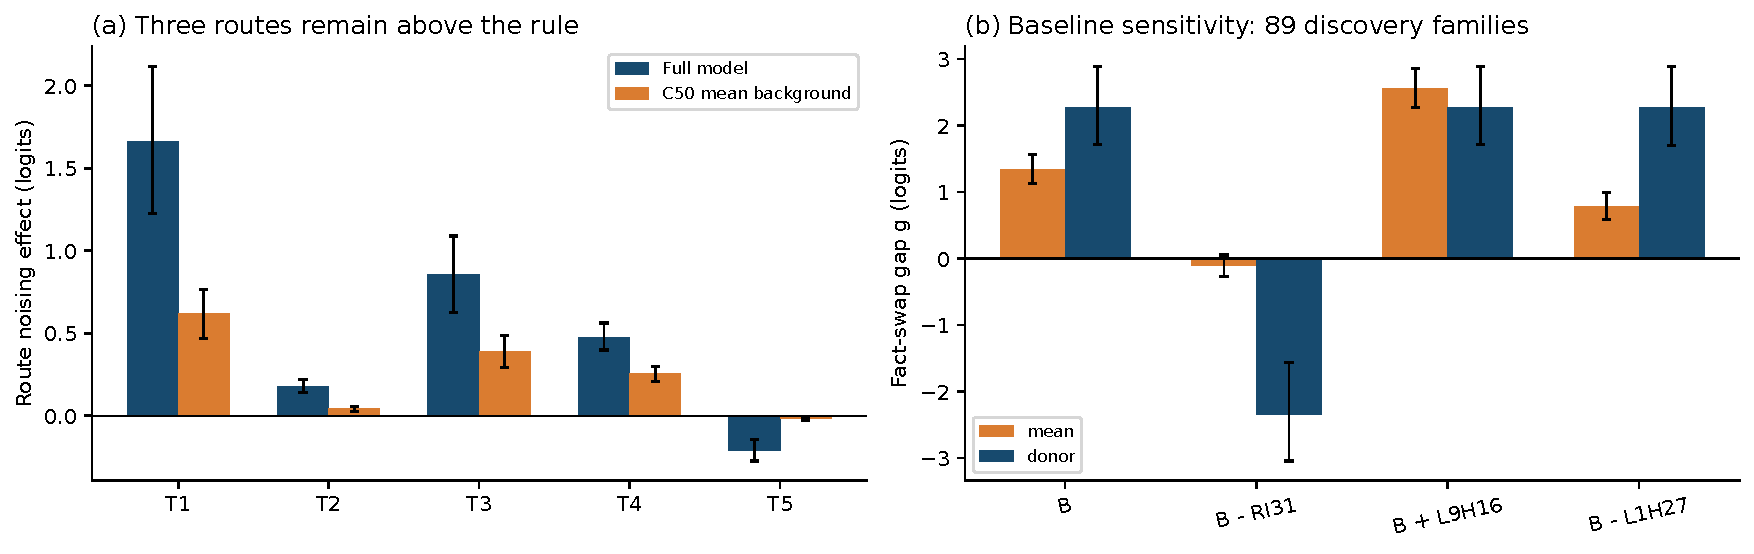
\includegraphics[width=\textwidth]{routes_and_baselines.pdf}
\caption{Background dependence. (a) Route effects in full and B on the core
families, with recomputed intervals. (b) Extension gaps under means and paired
donors, with intervals from the supplied summary. Intervals on these individual
bars are not intervals for differences between bars.}
\label{fig:baseline}
\end{figure}

\paragraph{Candidate effects shrink, while collective RI dependence persists.}
Table~\ref{tab:sensitivity} subtracts the matched configuration means in
Table~\ref{tab:extension}. Individual contributions under donor replacement are
very small but positive; neither is exactly zero. In contrast, the collective
RI effect grows under donor replacement. B without RI has a negative gap under
donors, so restoring the RI group shifts behaviour toward the current facts.
No paired interval is reconstructed for these 89-family differences because
the required family vectors are absent from the local package.

\begin{table}[htbp]\centering\small
\begin{tabular}{@{}lrr@{}}
\toprule
Contribution & Mean $\Delta g$ & Donor $\Delta g$ \\
\midrule
L9H16 & +1.210 & +0.003 \\
L1H27 & +0.552 & +0.006 \\
R(B) & +1.448 & +4.615 \\
\bottomrule
\end{tabular}

\caption{Functional changes in the original-axis gap. L9H16 compares $B+h$ to B;
L1H27 compares B to $B-h$; the group compares B to $B-R(B)$. These are
89-family $\Delta g$ values, not the 20-family four-cell $\Delta b$.}
\label{tab:sensitivity}
\end{table}

The non-RI remainder is not inert under means: its gaps are $+5.556$ and
$-5.767$ by order, cancelling to $-0.106$. Removing RI largely eliminates the
\emph{order-averaged, correctly oriented} fact contrast while substantial
order-dependent activity remains. The group result also does not show which
of its 31 members carries that effect.

Changing the replacement baseline changes both the background and the value used
when a candidate is absent. The disappearance of a toggle effect therefore
demonstrates baseline dependence; it does not identify redundancy as its cause.
Neither replacing heads by means nor by opposite-fact outputs silences the
remaining network. The observed shift could reflect preserved information,
different interactions or compensation; the current measurements do not choose
between these explanations.

\section{Corrections to the supplied interpretation}
Most reported numerical means reproduce. The main revisions concern mechanistic
conclusions and a few scope/precision errors, summarized here.
\small
\begin{longtable}{@{}p{5.6cm}p{10.4cm}@{}}
\toprule
Original interpretation & Supported replacement \\
\midrule
\endhead
``The two candidates are not route members; their effect is additive/parallel.'' &
No tested Gamma crosses the effect rule. The mechanism is unresolved; attachments
were not run. Below-threshold interaction is not a serial-membership test.\\
\addlinespace
``Question-conditioned selection is outside C50.'' &
C50 with the remainder mean-replaced fails query-conditioned behaviour. The
contrast does not locate the missing computation or exclude distributed
interactions involving C50 itself.\\
\addlinespace
``The non-RI remainder is inert.'' &
Its mean gap nearly cancels across opposite order effects. It remains strongly
order-sensitive.\\
\addlinespace
``The collective effect belongs to already strong RI heads.'' &
Collective removal does not identify its individual contributors. L8H15 itself
was below the earlier 0.3-logit strong-head threshold.\\
\addlinespace
``C50 contains every RI candidate.'' &
C50 contains 31 of the original 59, and five of the six new candidates. L9H16 is
added separately.\\
\addlinespace
``No candidate changes any accuracy.'' &
Candidate accuracy is unchanged; L1H27 improves full-vocabulary top-token
accuracy by five points in two core conditions.\\
\addlinespace
``All relative Gamma effects are at most 5\%.'' &
This holds for eligible pairs with the stated denominator, not for weak routes.
The absolute-effect rule is the primary criterion.\\
\addlinespace
``The donor effects disappear / are symmetric.'' &
The candidate effects become very small positive values. B has positive gaps in
both orders, but 3.141 and 1.403 are not symmetric magnitudes.\\
\addlinespace
``The empty model is a constant output / true zero.'' &
The core fact/query contrasts are zero; margins vary between families and the
extension gap is 0.018.\\
\addlinespace
``Four first-anchor name-gap leaders do nothing.'' &
The four candidates span different diagnostics, including last-anchor selection.
Their effects are below the frozen rule, not necessarily zero.\\
\bottomrule
\end{longtable}
\normalsize

\section{What is frozen and what remains unvalidated}
The freeze is internally consistent and selects only L9H16 and L1H27 for
behavioural follow-up. The actual held-out suite therefore contains six mean
configurations (full, empty, B, $B-R(B)$, $B+\mathrm{L9H16}$ and
$B-\mathrm{L1H27}$) on four cells, and four donor configurations on the original
two cells. There are no Gamma or attachment jobs. At 87 families and two orders,
this is
\[
6\times87\times2\times4+4\times87\times2\times2=5{,}568
\]
scored behavioural endpoints before reuse; donor captures, loading and gates
are additional. The supplied analysis's seven/five configuration counts are
protocol maxima, not the suite selected by this run.

The extension is not independent replication: its 89 families include the 20
core families. The extension summary mixes 89-family original-axis statistics
with 20-family changed-query statistics; the single \file{families} field does
not describe every field in that object. The unselected candidates, all Gamma
screening results, and the nested-route comparison remain discovery findings.
No final held-out outcome label is assigned here; the observed baseline
sensitivity will need to accompany any subsequent validation result.

\section{Conclusions}
The final discovery experiment separates three outcomes that should not be
collapsed into a single verdict on RI.

\textbf{Known RI participation remains supported.} Three communications survive
inside the partial retained background. In particular, the nested-route contrast
supports L18H19's conditional contribution, and the L8H15 V route remains
coherent. Collective RI removal changes behaviour under both replacement
baselines, although its size and the remaining behaviour differ substantially.

\textbf{Additional functional participants do not yet have new route assignments.}
L9H16 and L1H27 improve the four-condition contrast under means, consistently
across the core families. Their donor-baseline effects are much smaller, and
none of the measured candidate--route interactions meets the planned rule.
The result is selective, background-dependent functional participation with
unresolved connections, not evidence that these heads are useless or necessarily
parallel to the known routes.

\textbf{The measured head collection is not a sufficient retained explanation.}
Preserving all previously strong heads and the expanded RI subset does not
preserve the task under the declared masking intervention. The first-chain bias
and small query contrast show the missing behavioural property directly.
The evidence supports causal components and communications involved in contextual
relation use, while the complete computation is not captured by C33 or C50.
This distinguishes failure of a retained mask from failure of the previously
measured routes, and failure of the new RI search from absence of RI participation.

\appendix
\section{Provenance and reproducibility}
The source analysis was preserved without edits. The independent audit and
derived files are in \file{results/stage4_s45_review_20260927/}. The report's
tables and vector figures are generated from the audited exports.
\begin{itemize}
\item Core data: \file{analysis/stage_a/core_behavior.csv} and
\file{analysis/stage_b/core_behavior_stage_b.csv}.
\item Route data: \file{analysis/stage_c/core_route_effects.csv}; every stored
effect equals intact minus endpoint margin, and all eight backgrounds have
five routes by 40 pairs.
\item Extension: \file{analysis/full_discovery/extension_summary.json}; its
family-level CSV retains only the core four-cell population.
\item Decisions: \file{B_decision.json}, \file{frozen_selection.json},
\file{freeze_manifest.json}, \file{pipeline_done.json}, and
\file{ri_membership_ledger.csv}.
\item Reproduction: \file{audit_s45.py}, \file{build_tables.py},
\file{checks.json} and \file{audit_summary.json}.
\end{itemize}
To extend the independent audit to every 89-family endpoint and to top-token
outcomes, the original worker chunks, their checksums and the mean-bank manifest
must be restored. Their absence limits the local verification depth; it does not
by itself indicate an error in the recorded run.
\end{document}
